% created on 2019-12-13
% @author : bmazoyer

%% Lines to compile only this capter
\documentclass[11pt, twoside, a4paper, openright]{report}
\usepackage[utf8]{inputenc}
% \DeclareUnicodeCharacter{223C}{~}

%Bibliography style
% \usepackage[square, numbers]{natbib}
% \usepackage[round]{natbib}
% \usepackage{biblatex}
% \bibliographystyle{unsrtnat}
% \bibliographystyle{unsrt}
% \bibliographystyle{plain}
% \bibliographystyle{aa}
% \usepackage[backend=bibtex,style=authoryear,natbib=true]{biblatex} 
\usepackage[
backend=biber,
style=authoryear,
citestyle=authoryear,
url=false
]{biblatex}
\addbibresource{../source/library.bib}

\usepackage[T1]{fontenc}
\usepackage[french]{babel}
\usepackage{csquotes}  % used for citations (recommended when using biblatex)
%\usepackage{helvet}
%\renewcommand{\familydefault}{\sfdefault}
\usepackage{mathptmx}
\usepackage{amssymb}
\usepackage{geometry} 
\usepackage{xcolor}
\usepackage[absolute,overlay]{textpos}
\usepackage{graphicx}
\usepackage{lipsum}
\usepackage[explicit]{titlesec}
\usepackage{lmodern}
\usepackage{color}
\usepackage{array}
\usepackage{mathtools}
\usepackage{caption}
\usepackage{multicol}
\usepackage{booktabs}
\usepackage{enumitem}
\usepackage{hyperref}
\usepackage{afterpage}
\usepackage{emptypage}
\usepackage{setspace}
\usepackage{pgffor}
    \setlength{\columnseprule}{0pt}
    \setlength\columnsep{10pt}
\usepackage[francais,nohints]{minitoc}
    \setcounter{minitocdepth}{3}
 
 %https://la-bibliotex.fr/2019/02/03/ecrire-les-nombres-et-les-unites-avec-latex/   
\usepackage{siunitx}
% \sisetup{
%     detect-all,
%      output-decimal-marker={,},
%      group-minimum-digits = 3,
%      group-separator={~},
%      number-unit-separator={~},
%      inter-unit-product={~},
%      list-separator = {, },
%      list-final-separator = { et },
%      range-phrase = --,
%      separate-uncertainty = true,
%      multi-part-units = single,
%      list-units = single,
%      range-units = single
%     }
\usepackage{physics}
\usepackage{isotope}

\usepackage[perpage]{footmisc} % to reset the counter of footnote each page

    
\usepackage{fancyhdr}			% Entête et pieds de page. Doit être placé APRES geometry
\pagestyle{fancy}		% Indique que le style de la page sera justement fancy
%\lfoot[\thepage]{} 		% gauche du pied de page
%\cfoot{} 			% milieu du pied de page
%\rfoot[]{\thepage} 
\fancyfoot{} % vide le pied~de~page
\fancyfoot[LE,RO]{\thepage}
\fancyfoot[LO,CE]{}% droite du pied de page
\fancyhead{}	
\fancyhead[LE]{\leftmark}	
\fancyhead[RO]{\rightmark}

\fancypagestyle{plain}{%
\fancyhf{} % vide l’en-tête et le pied~de~page.
\fancyfoot[LE,RO]{\thepage} % numéro de la page en cours en gras% et centré en pied~de~page.
\renewcommand{\headrulewidth}{0pt}
\renewcommand{\footrulewidth}{0pt}}



% Premiere page des chapitres
\newlength\chapnumb
\setlength\chapnumb{3cm}
 
\titleformat{\chapter}[block] {
  \normalfont}{}{0pt} { %police
    \parbox[b]{\chapnumb}{
      \fontsize{120}{110}\selectfont\thechapter} %taille du chiffre
      \parbox[b]{\dimexpr\textwidth-\chapnumb\relax}{
        \raggedleft 
        \hfill{\bfseries\Huge#1}\\ %taille du titre
        \rule{\dimexpr\textwidth-\chapnumb\relax}{0.4pt} %ligne de separation
  }
}
 
 %premiere page chapitre non numerote (remerciement, table des matieres ...)
 
\titleformat{name=\chapter,numberless}[block]
{\normalfont}{}{0pt}
{   
    \parbox[b]{\dimexpr\textwidth}{%   
    \hfill{\bfseries\Huge#1}\\
  \rule{\dimexpr\textwidth}{0.4pt}}}
    
 %   \titleformat{name=\chapter,numberless}[block]
%{\normalfont}{}{0pt}
%{\parbox[b]{\chapnumb}{%
%   \mbox{}}%
%  \parbox[b]{\dimexpr\textwidth-\chapnumb\relax}{%
%    \raggedleft%
%    \hfill{\bfseries\Huge#1}\\
%    \rule{\dimexpr\textwidth-\chapnumb\relax}{0.4pt}}}


%%%    SIunitx
\sisetup{locale = FR,
  % inter-unit-product=\ensuremath{\cdot},
  inter-unit-product=\ensuremath{\,},
  per-mode=reciprocal,
  separate-uncertainty = true,
  detect-all
}
\DeclareSIUnit{\Mpc}{Mpc}
\DeclareSIUnit{\kpc}{kpc}
\DeclareSIUnit{\Gpc}{Gpc}
\DeclareSIUnit{\h}{\textit{h}~}
\DeclareSIUnit{\perh}{\textit{h}^{-1}\,}

%%% Geometry
\geometry{
left=20mm,
top=30mm,
right=20mm,
bottom=30mm
}

%%% Color
\definecolor{bordeau}{rgb}{0.3515625,0,0.234375}

%%% Commands
\newcommand{\Nmocks}{\num{30}}
\newcommand{\hMpc}{h^{-1}\,\mathrm{Mpc}}
\newcommand{\hGpc}{h^{-1}\,\mathrm{Gpc}}
\newcommand{\kms}{\mathrm{km\,s^{-1}}}

\newcommand{\lya}{Ly$\alpha$}
\newcommand{\lyb}{Ly$\beta$}
\newcommand{\lyalya}{Ly$\alpha$(Ly$\alpha$)}
\newcommand{\lyalyb}{Ly$\alpha$(Ly$\beta$)}

\newcommand{\lrf}{\lambda_{\rm RF}}
\newcommand{\kpar}{k_{\parallel}}
\newcommand{\apar}{\alpha_{\parallel}}
\newcommand{\rpar}{r_{\parallel}}
\newcommand{\aperp}{\alpha_{\perp}}
\newcommand{\rperp}{r_{\perp}}
\newcommand{\kperp}{k_{\perp}}

\newcommand{\blya}{b_{\rm Ly\alpha}}
\newcommand{\betalya}{\beta_{\rm Ly\alpha}}
\newcommand{\blyb}{b_{\rm Ly\alpha}}
\newcommand{\betalyb}{\beta_{\rm Ly\beta}}
\newcommand{\dlya}{d_{\rm Ly\alpha}}
\newcommand{\bhcd}{b_{\rm HCD}}
\newcommand{\betahcd}{\beta_{\rm HCD}}
\newcommand{\Fhcd}{F_{\rm HCD}}
\newcommand{\Lhcd}{L_{\rm HCD}}

\newcommand{\imin}{i_{\rm min}}
\newcommand{\imax}{i_{\rm max}}
\newcommand{\jmin}{j_{\rm min}}
\newcommand{\jmax}{j_{\rm max}}

\newcommand{\xioned}{\xi_{\rm 1d}}
\newcommand{\DHub}{D_{H}}
\newcommand{\DM}{D_{M}}

\newcommand{\omegam}{\Omega_M}
\newcommand{\omegac}{\Omega_C}
\newcommand{\omegab}{\Omega_B}
\newcommand{\omegan}{\Omega_\nu}
\newcommand{\omegal}{\Omega_\Lambda}
\newcommand{\omegak}{\Omega_k}
\newcommand{\orad}{\Omega_R}
\newcommand{\ogam}{\Omega_\gamma}
\newcommand{\lcdm}{$\Lambda$CDM}

\newcommand{\picca}{\texttt{picca}}

%%% Rem's command
\newcommand\blankpage{%
    \null
    \thispagestyle{empty}%
    \addtocounter{page}{-1}%
    \newpage}
  
% Command to set up a particular alignment for a cell in tabular :
% \myalign{c}{foo} for instance
\newcommand*{\myalign}[2]{\multicolumn{1}{#1}{#2}}
 
\renewcommand{\thesection}{\arabic{section}}

% Romain
\newcommand{\cRM}[1]{\MakeUppercase{\romannumeral #1}}	% Capital
\newcommand{\cRm}[1]{\textsc{\romannumeral #1}}	% Petit majuscule
\newcommand{\crm}[1]{\romannumeral #1}
% Siècle %
\newcommand{\siecle}[1]{\cRm{#1}\textsuperscript{e}~siècle}



% Thesis title
\newcommand{\PhDTitle}{Les forêts \lya{} du relevé eBOSS : comprendre les fonctions de corrélation et les systématiques} 

% Name
\newcommand{\PhDname}{Thomas Etourneau} 

% Change this variable if you add or remove chapters
\newcommand*{\NumOfChapters}{6}

% Change this variable if you add or remove appendices
\newcommand*{\NumOfAppendices}{2}

% PDF metadata
\hypersetup{
	pdfauthor={\PhDname},
	pdfsubject={Manuscrit de thèse de doctorat},
	pdftitle={\PhDTitle}
}


\begin{document}
%%

\graphicspath{ {../figures/data_ana/} }

\chapter{Analyse des données et résultats}
\minitoc
\newpage
\thispagestyle{fancy}

Dans ce chapitre, nous présentons les diverses analyses que nous avons mené sur les données, avec les mocks comme support de référence.
Un élément clé à la construction des mocks a été de déterminer quels paramètres \lya{} nous souhaitions avoir dans nos mocks. En produisant l'analyse des données DR16 en quatre bins en redshift, nous nous sommes rendus compte que les paramètres \lya{} obtenus dépendaient fortement de la modélisation des HCD. Nous avons dû faire un choix quant à cette modélisation.
Nous présentons donc d'abord l'analyse des données qui a servi de référence pour l'ajustement des paramètres des mocks. Puis, nous discutons la modélisation des HCD et présentons des modélisations alternatives.
\#prov finir de donner les autres sections



\section{L'analyse des données DR16}
L'analyse des données finale d'eBOSS (DR16), dont nous avons déjà parlé et qui est présentée dans \citet{prov}, analyse les fonctions de corrélation \lya(\lya{})$\times$\lya{}(\lya{}), \lya{}(\lya{})$\times$\lya{}(\lyb{}), \lya{}(\lya{})$\times$QSO et \lya{}(\lyb{})$\times$QSO. Ces fonctions de corrélation sont construites sur l'ensemble des données, les paramètres ajustés sont donc donnés uniquement pour le redshift effectif $z_{\mathrm{eff}} = \num{2.334}$ de la mesure. L'appendice F de \citet{prov} présente cependant l'analyse des données DR16 dans deux bins en redshift. Mais ces deux bins ne sont pas suffisant pour estimer les paramètres \lya{} dans toute la gamme en redshift $1.9 < z  < 3.6$.
% Afin d'estimer $b_{\mathrm{Ly}\alpha}(z)$ et $\beta_{\mathrm{Ly}\alpha}(z)$ dans cette gamme, nous avons calculé la fonction de corrélation \lya{}$\times$\lya{} dans quatres bins en redshift.
Afin d'estimer $b_{\mathrm{Ly}\alpha}(z)$ et $\beta_{\mathrm{Ly}\alpha}(z)$ dans cette gamme, nous avons reproduit cette analyse dans quatres bins en redshift. De manière à limiter les potentielles systématiques, nous nous limitons à l'analyse de la fonction de corrélation \lya{}(\lya{})$\times$\lya{}(\lya{}) (abrégée en \lya{}$\times$\lya{} dans la suite de ce chapitre).
% Pour chacun des bins, nous calculons la fonction de corrélation pour les forêts dont le redshift du quasar se trouve dans l'intervale en redshift considéré. Ceci permet d'éviter des corrélations  (voir Appendice B de \citet{Agathe2019a}).
% Pour constituer chacun des bins en redshift, plutôt que de considérer le redshift effectif de chaque paire de pixels, nous divisons l'échantillon de forêts selon le redshift des quasars. Ceci nous permet d'éviter les corrélations induites
Pour constituer chacun des bins en redshift, nous pourions séparer les paires de pixels selon leur redshift effectif. Cependant, à cause de l'ajustement du continuum, cette stratégie induit des corrélations parasites lorsqu'une forêt se trouve dans deux bins en redshift à la fois. Pour palier ce problème, nous divisons l'échantillon de forêts selon le redshift des quasars (voir Appendice B de \citet{Agathe2019a}).
Les quatres intervales choisis pour construire les bins en redshift sont $[\num{0}\,;\num{2.35}]$, $[\num{2.35}\,;\num{2.65}]$, $[\num{2.65}\,;\num{3.05}]$ et $[\num{3.05}\,;\num{10}]$.
% Nous calculons aussi la matrice de distorsion dans chacun de ces bins.
Dans chacun des bins, nous calculons la fonction de corrélation \lya{}$\times$\lya{}, ainsi que la matrice de distorsion associée.
Enfin, nous procédons à l'ajustement des quatres fonctions de corrélation. Le modèle utilisé pour cet ajustement est le même que celui utilisé pour l'analyse des données finale d'eBOSS \citep{prov}, il est présenté dans la section~\ref{subsec:model_donnees}.
Chacune des fonctions de corrélation est ajustée au redshift effectif de la mesure. Ces redshifts sont $z_1 = \num{2.136}$, $z_2 = \num{2.276}$, $z_3 = \num{2.551}$ et $z_4 = \num{2.914}$.

\begin{figure}
  \centering
  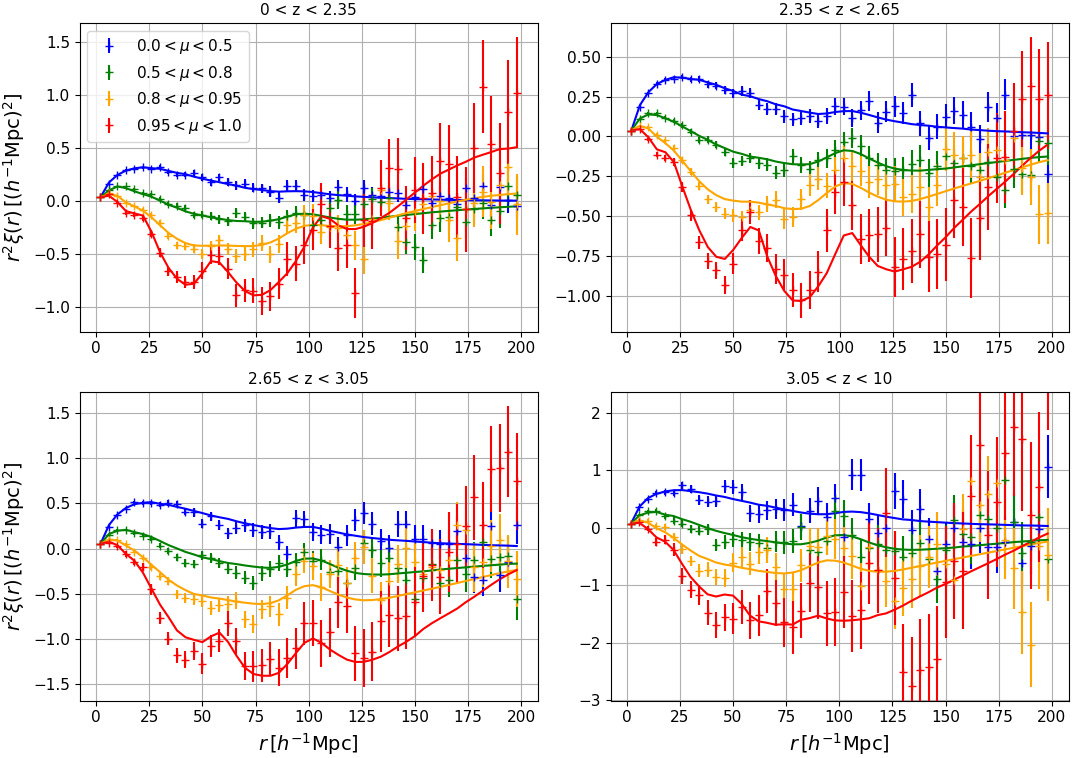
\includegraphics[scale=0.5]{dr16_4bins}
  \caption{Fonctions de corrélation \lya{}$\times$\lya{} dans chacun des bins en redshift de l'analyse. Les courbes en trait plein donne le meilleur ajustement du modèle obtenu avec \texttt{picca}. Chaque graphique correspond à un bin en redshift. Pour chacun des bins, la fonction de corrélation et l'ajustement sont montrées dans quatre bins en $\mu$.}
  \label{fig:dr16_4bins}
\end{figure}

\begin{table}[]
  \centering
  \caption{Résultats de l'ajustement fait avec \texttt{picca} des fonctions de corrélation \lya{}$\times$\lya{} calculées sur les données DR16. Chaque colonne donne le résultat de l'ajustement d'un bin en redshift. La première section du tableau donne les paramètres du modèle qui sont ajustés. La seconde donne le $\chi^2$. Le nombre de bins sur lesquels le modèle est ajusté est $N_{bin} = \num{1590}$. Le modèle comporte \num{13} paramètres libres. Enfin, la dernière section donne le biais et le biais effectif du \lya{}. Ils sont reliés aux paramètres $b_{\eta, \mathrm{Ly}\alpha}$ et $\beta_{\mathrm{Ly}\alpha}$ par les équations~\ref{eq:def_bias} et~\ref{eq:def_bias_eff}.}
  \label{tab:dr16_4bins}
  \begin{tabular}{lllll}
    \toprule
    Paramètre  & $\num{0} < z < \num{2.35}$ & $\num{2.35} < z < \num{2.65}$ & $\num{2.65} < z < \num{3.05}$ & $\num{3.05} < z < \num{10}$ \\
    \midrule
    % $\apar{}$ & 1.0626413422656635 +/- 0.06560781661781079 & 1.0188646800560925 +/- 0.041362422911403685 & 1.029148212201299 +/- 0.07242396192712802 & 1.1200171298229007 +/- 0.08091370899309824 \\
    % $\aper{}$ & 1.0632375535901253 +/- 0.10810794059323114 & 0.9652958910718991 +/- 0.057180394974236104 & 1.0159330757036005 +/- 0.05784775528375763 0.9255146850435335 +/- 0.07206257341759192 \\
    % $b_{\eta, \mathrm{Ly}\alpha}$ & -0.1795977211203897 +/- 0.005769053847991895 & -0.19377778657236358 +/- 0.00526939132784233 & -0.2236876829818197 +/- 0.008421287322167362 & -0.2928514012382003 +/- 0.018740373333761263 \\
    % $\beta_{\mathrm{Ly}\alpha}$ & 2.093809306317262 +/- 0.210449292900992 & 1.7112686242434043 +/- 0.13322965498374356 & 1.4274033068601393 +/- 0.13841133835520955 & 1.264422978848562 +/- 0.19412583530626168 \\
    % $10^3 b_{\eta, SiII(1190)}$ & -0.0018292445000232958 +/- 0.0010951582472295686 & -0.003656308599416015 +/- 0.0006752880865250276 & -0.002801629741142273 +/- 0.0010118710088140865 & 0.00036032759305010395 +/- 0.0016376260200395207 \\
    % $10^3 b_{\eta, SiII(1193)}$ & -0.004830928957010919 +/- 0.001100315153087375 & -0.0019362727878605114 +/- 0.0006919289269201215 & -0.0007847568940101366 +/- 0.0009691126424570403 & -0.002131181997407055 +/- 0.0017224737321217046 \\
    % $10^3 b_{\eta, SiII(1260)}$ & -0.003375467125024695 +/- 0.0013329581881429706 &  -0.001969961682619123 +/- 0.000795815740207674 & -0.001317200522029868 +/- 0.0010526150274975418 & 0.0008965020540008499 +/- 0.001791480805493678 \\
    % $10^3 b_{\eta, SiIII(1207)}$ &  -0.007865921480598285 +/- 0.0011034826815558326 & -0.004523595559873886 +/- 0.0007456098975624773 & -0.0021082960921853036 +/- 0.001047671905738136 & -0.0028969289782045586 +/- 0.001740041127658313 \\
    % $10^3 b_{\eta, CIV(eff)}$ & -0.004767305959965107 +/- 0.002544174250674547 & -0.005150878411363191 +/- 0.002643560029682246 & -0.005060576315171872 +/- 0.0026177990462492584 & -0.005022340903756195 +/- 0.002605282928692776 \\
    % $b_{\textsc{HCD}}$ & -0.05959772317290102 +/- 0.007001888877137152 & -0.04517388629736585 +/- 0.0060459072913988665 & -0.06651201389736294 +/- 0.010015445096663855 & -0.022781727665758256 +/- 0.021820968368492788 \\
    % $\beta_{\textsc{HCD}}$ & 0.5513755924633041 +/- 0.08641628187515504 & 0.55971852703097 +/- 0.08649826856663473 & 1.4274033068601393 +/- 0.13841133835520955 & 0.5026113732660472 +/- 0.08990286553465421 \\
    % $10^2 A_{sky}$ & 0.015852430760394755 +/- 0.0009832458229809115 & 0.008702223782589641 +/- 0.000816825935201006 & 0.007285381419552714 +/- 0.0013334299368094303 & 0.006448552548337415 +/- 0.0033839253887543966 \\
    % $\sigma_{sky}$ & 32.542936141293126 +/- 1.7910999585024947 & 31.590693919063543 +/- 2.5612829757179214 & 31.930967631996463 +/- 4.270238324140993
    % \bottomrule & 34.1693831220765 +/- 16.09450395736028 \\

    % $\apar{}$ & 1.0626413422656635 +/- 0.06560781661781079 & 1.0188646800560925 +/- 0.041362422911403685 & 1.029148212201299 +/- 0.07242396192712802 & 1.1200171298229007 +/- 0.08091370899309824 \\
    % $\aper{}$ & 1.0632375535901253 +/- 0.10810794059323114 & 0.9652958910718991 +/- 0.057180394974236104 & 1.0159330757036005 +/- 0.05784775528375763 0.9255146850435335 +/- 0.07206257341759192 \\
    % $b_{\eta, \mathrm{Ly}\alpha}$ & -0.1795977211203897 +/- 0.005769053847991895 & -0.19377778657236358 +/- 0.00526939132784233 & -0.2236876829818197 +/- 0.008421287322167362 & -0.2928514012382003 +/- 0.018740373333761263 \\
    % $\beta_{\mathrm{Ly}\alpha}$ & 2.093809306317262 +/- 0.210449292900992 & 1.7112686242434043 +/- 0.13322965498374356 & 1.4274033068601393 +/- 0.13841133835520955 & 1.264422978848562 +/- 0.19412583530626168 \\
    % $10^3 b_{\eta, SiII(1190)}$ & -1.8292445000232958 +/- 1.0951582472295686 & -3.656308599416015 +/- 0.6752880865250276 & -2.801629741142273 +/- 1.0118710088140865 & 0.36032759305010395 +/- 1.6376260200395207 \\
    % $10^3 b_{\eta, SiII(1193)}$ & -4.830928957010919 +/- 1.100315153087375 & -1.9362727878605114 +/- 0.6919289269201215 & -0.7847568940101366 +/- 0.9691126424570403 & -2.131181997407055 +/- 1.7224737321217046 \\
    % $10^3 b_{\eta, SiII(1260)}$ & -3.375467125024695 +/- 1.3329581881429706 &  -1.969961682619123 +/- 0.795815740207674 & -1.317200522029868 +/- 1.0526150274975418 & 0.8965020540008499 +/- 1.791480805493678 \\
    % $10^3 b_{\eta, SiIII(1207)}$ &  -7.865921480598285 +/- 1.1034826815558326 & -4.523595559873886 +/- 0.7456098975624773 & -2.1082960921853036 +/- 1.047671905738136 & -2.8969289782045586 +/- 1.740041127658313 \\
    % $10^3 b_{\eta, CIV(eff)}$ & -4.767305959965107 +/- 2.544174250674547 & -5.150878411363191 +/- 2.643560029682246 & -5.060576315171872 +/- 2.6177990462492584 & -5.022340903756195 +/- 2.605282928692776 \\
    % $b_{\textsc{HCD}}$ & -0.05959772317290102 +/- 0.007001888877137152 & -0.04517388629736585 +/- 0.0060459072913988665 & -0.06651201389736294 +/- 0.010015445096663855 & -0.022781727665758256 +/- 0.021820968368492788 \\
    % $\beta_{\textsc{HCD}}$ & 0.5513755924633041 +/- 0.08641628187515504 & 0.55971852703097 +/- 0.08649826856663473 & 1.4274033068601393 +/- 0.13841133835520955 & 0.5026113732660472 +/- 0.08990286553465421 \\
    % $10^2 A_{sky}$ & 1.5852430760394755 +/- 0.09832458229809115 & 0.8702223782589641 +/- 0.0816825935201006 & 0.7285381419552714 +/- 0.13334299368094303 & 0.6448552548337415 +/- 0.33839253887543966 \\
    % $\sigma_{sky}$ & 32.542936141293126 +/- 1.7910999585024947 & 31.590693919063543 +/- 2.5612829757179214 & 31.930967631996463 +/- 4.270238324140993
    % \bottomrule & 34.1693831220765 +/- 16.09450395736028 \\

    $\apar{} $ & $ 1.063 \pm 0.066 $ & $ 1.019 \pm 0.041 $ & $ 1.029 \pm 0.072 $ & $ 1.120 \pm 0.081 $ \\
    $\aperp{} $ & $ 1.063 \pm 0.108 $ & $ 0.965 \pm 0.057 $ & $ 1.016 \pm 0.058 $ & $ 0.926 \pm 0.072 $ \\
    $b_{\eta, \mathrm{Ly}\alpha} $ & $ -0.1796 \pm 0.0058 $ & $ -0.1938 \pm 0.0053 $ & $ -0.2239 \pm 0.0084 $ & $ -0.2929 \pm 0.0187 $ \\
    $\beta_{\mathrm{Ly}\alpha} $ & $ 2.094 \pm 0.210 $ & $ 1.711 \pm 0.133 $ & $ 1.427 \pm 0.138 $ & $ 1.264 \pm 0.194 $ \\
    $10^3 b_{\eta, SiII(1190)} $ & $ -1.83 \pm 1.10 $ & $ -3.66 \pm 0.68 $ & $ -2.80 \pm 1.01 $ & $ 0.36 \pm 1.64 $ \\
    $10^3 b_{\eta, SiII(1193)} $ & $ -4.83 \pm 1.10 $ & $ -1.94 \pm 0.69 $ & $ -0.78 \pm 0.97 $ & $ -2.13 \pm 1.72 $\\
    $10^3 b_{\eta, SiII(1260)} $ & $ -3.38 \pm 1.33 $ & $  -1.97 \pm 0.80 $ & $ -1.32 \pm 1.05 $ & $ 0.90 \pm 1.79 $\\
    $10^3 b_{\eta, SiIII(1207)} $ & $  -7.87 \pm 1.10 $ & $ -4.52 \pm 0.74 $ & $ -2.11 \pm 1.05 $ & $ -2.90 \pm 1.74 $\\
    $10^3 b_{\eta, CIV(\mathrm{eff})} $ & $ -4.77 \pm 2.54 $ & $ -5.15 \pm 2.64 $ & $ -5.06 \pm 2.62 $ & $ -5.02 \pm 2.61 $\\
    $b_{\textsc{HCD}} $ & $ -0.0596 \pm 0.0070 $ & $ -0.0452 \pm 0.0060 $ & $ -0.0665 \pm 0.0100 $ & $ -0.0228 \pm 0.0218 $\\
    $\beta_{\textsc{HCD}} $ & $ 0.551 \pm 0.086 $ & $ 0.560 \pm 0.086 $ & $ 0.508 \pm 0.088 $ & $ 0.503 \pm 0.090 $\\
    $10^2 A_{sky} $ & $ 1.585 \pm 0.098 $ & $ 0.870 \pm 0.082 $ & $ 0.729 \pm 0.133 $ & $ 0.645 \pm 0.338 $\\
    $\sigma_{sky} $ & $ 32.5 \pm 1.7 $ & $ 31.6 \pm 2.6 $ & $ 31.9 \pm 4.3 $ & $ 34.2 \pm 16.1 $\\
    \midrule
    $\chi^2$ & 1568.33 & 1512.33 & 1680.82 & 1674.59 \\
    \midrule
    $b_{\mathrm{Ly}\alpha} $ & $ -0.0832 \pm -0.0065 $ & $ -0.1099 \pm -0.0063 $ & $ -0.1521 \pm -0.01025 $ & $ -0.2248 \pm -0.0230 $\\
    $b_{\mathrm{eff}, \mathrm{Ly}\alpha} $ & $ -0.1506 \pm 0.0046 $ & $ -0.1814 \pm 0.0045 $ & $ -0.2336 \pm 0.0074 $ & $ -0.3305 \pm 0.0169 $\\
    \bottomrule
\end{tabular}
\end{table}


La figure~\ref{prov} présente les fonctions de corrélation et leur modèle ajusté dans chacun des bins en redshift. Les différents graphiques montre les différents bins en redshift. Dans chaque graphique, la fonction de corrélation est affichée dans plusieurs bins en $\mu$. Le tableau~\ref{prov} donne le résultat de l'ajustement dans chacun des bins en redshift. La première section du tableau donne les paramètres ajustés, la deuxième donne le $\chi^2$ obtenu. Le nombre de bins dans lesquels la fonction de corrélation est ajusté est $N_{bin} = \num{1590}$, ce qui donne un nombre de degrés de liberté de $d.o.f. = \num{1590} - \num{13} = \num{1577}$. Enfin, la troisième colonne donne le biais et le biais effectif du \lya{}. Le biais $b_{\mathrm{Ly}\alpha} $ est obtenu comme
\begin{equation}
  \label{eq:def_bias}
  b_{\mathrm{Ly}\alpha}  = \frac{b_{\eta, \mathrm{Ly}\alpha} f}{\beta_{\mathrm{Ly}\alpha}} \; .
\end{equation}
Le biais effectif $b_{\mathrm{eff}, \mathrm{Ly}\alpha} $ est défini comme
\begin{equation}
  \label{eq:def_bias_eff}
  b_{\mathrm{eff}, \mathrm{Ly}\alpha} = b_{\mathrm{Ly}\alpha} \sqrt{1 + \frac{2}{3} \beta_{\mathrm{Ly}\alpha} + \frac{1}{5} \beta_{\mathrm{Ly}\alpha}^2} \; .
\end{equation}
Il est sensible à l'amplitude de la fonction de corrélation, et est moins corrélé avec $\beta_{\mathrm{Ly}\alpha}$ que l'est $b_{\eta, \mathrm{Ly}\alpha}$ ou $b_{\mathrm{Ly}\alpha}$.


Une fois avoir produit ces ajustements, nous avons regardé la corrélation des paramètres 


\bibliography{../source/library}
\end{document}
